\chapter{スーパーバイザ制御理論}
%またスーパーバイザ制御とは,制御対象に対して,制御要求を満たさない遷移をしてしまう事象を起こらないように禁止するシステムである.
この章では,離散事象システムとオートマトン,およびスーパーバイザ制御の計算方法を解説する.

\section{オートマトン}

\subsection{有限オートマトンの基本}

離散事象システムとは,離散的な状態集合を持つ事象駆動型システムである\cite{DES}.事象が生起すると,その事象に依存して状態が変わり,その状態が時間的に持続するのが特徴である.
オペーションシステム,データベースシステム,通信システム,生産システム,シーケンス制御システムなどが離散事象システムとみなせるいい例である\cite{des_example}.

離散事象システムのモデリングには有限オートマトンが適している.有限オートマトンとは有限個の状態と事象が定義されている動的システムのことである.生起した事象と状態遷移関数に従って,現在いる状態を遷移し連続する一連の動作(ふるまい)をモデリングする.

有限オートマトン$G$は次のように5つの要素から表される.
\begin{equation}
    G = (Q, \Sigma, \delta, q_{0}, Q_{m})
\end{equation}
ここで$Q$は状態の集合,$\Sigma$は事象の集合,$\delta$は状態遷移関数,$q_0\in Q$は初期状態,$Q_m\subseteq Q$は受理状態の集合を表している.状態遷移は$\delta(q,\sigma)$と書き,さらに状態$q$において事象$\sigma$が生起しうることを$\delta(q,\sigma)$が定義されているといい,以下のように表される.

$$\delta(q,\sigma)!$$

$k$個の事象$\sigma_i\in\Sigma(i=1,\cdots,k)$において,$s=\sigma_1 \cdots \sigma_k$とならべたものを事象列$s$と呼ぶ.また,事象列の事象の数を,事象列の長さといい,$\mid s\mid$と書くことで$s$の長さを表す.

$\Sigma$に含まれる事象で作られるすべての事象列の集合を$\Sigma^\ast$とかく.この$\Sigma^\ast$には,長さ0の事象列である空事象列$\epsilon$も含まれている.

状態遷移関数$\delta:Q\times\Sigma\rightarrow Q$
を
$\hat{\delta}:Q\times\mathrm{\Sigma}^\ast\rightarrow Q$
のように,以下の式の通りに拡張する.
\begin{eqnarray*}
    \hat{\delta}(q,\epsilon) &=& q\\
    \hat{\delta}(q,\sigma) &=& \delta(q,\sigma), q\in Q, \sigma\in\Sigma\\
    \hat{\delta}(q,s\sigma) &=& \delta(\hat{\delta}(q,s),\sigma), q\in Q, \sigma\in\Sigma, s\in\Sigma^\ast
\end{eqnarray*}
そして以後,$\hat{\delta}$のハットを省略して$\delta$とかく.


\subsection{言語}

$\Sigma^\ast$の任意の部分集合を事象集合$\Sigma$の言語$L$という.
\begin{equation}
    L\subseteq\Sigma^\ast
\end{equation}
ある集合を与えられたとき,その集合のすべての部分集合から構成される集合をべき集合という.そして$\Sigma^\ast$のべき集合を$Pwr(\Sigma^\ast)$とかき,$L$は以下のようにも記すことができる.

\begin{equation}
    L\in Pwr(\Sigma^\ast)
\end{equation}

事象列$s\in\Sigma^\ast$を$s=s_1 s_2$とかくことができる事象列$s_2\in\Sigma^\ast$が存在するとき事象列$s_1\in\Sigma^\ast$をsの接頭語とよぶ.言語$L$に含まれる事象列のすべての接頭語からなる言語$\overline{L}$を次のように表す.

\begin{equation}
    \overline{L} = \{ s_1 \in\Sigma^\ast\mid(\exists s_2 \in \Sigma^\ast) s_1 s_2\in L\}
\end{equation}

オートマトン$G$に対して,起こり得るすべての事象集合を$L(G)$と定義する.
\begin{equation}
    L(G) \coloneqq \{s\in \Sigma^\ast \mid \delta(q_0, s)! \}\subseteq\Sigma^\ast
\end{equation}
また,$L(G)$のうち,初期状態から受理状態まで遷移する事象列の集合を$L_m(G)$といい以下のように定義する.
\begin{equation}
    L_m(G) \coloneqq \{s\in L(G) \mid \delta(q_0, s) \in Q_m\} \subseteq L(G)
\end{equation}

$\overline{L_m(G)}=L(G)$が成り立つ場合にのみ, $G$はノンブロッキングだといえる.


\section{オートマトンの計算}

\subsection{自己ループ}

オートマトン$G = (Q, \Sigma, \delta, q_0, Q_m)$をおいたとき,$\Sigma^\prime \cap \Sigma=\emptyset$である事象の集合$\Sigma^\prime$との自己ループ$G_{sl}$は次のようなオートマトンとなる.
\begin{equation}
    G_{sl}=(Q,\Sigma\dot{\cup}\Sigma^\prime,\delta\dot{\cup}\delta^\prime,q_0,Q_m)
\end{equation}
ただし,$\delta^\prime\coloneqq\{[q,\sigma^\prime,q]\mid q\in Q,\sigma^\prime\in\Sigma^\prime\}$.つまり,自己ループというのは,もともと定義された$G$に関係のない事象$\sigma^\prime$が起こったとき,$G$は同じ状態に遷移するという操作(計算)のことである.


\subsection{自然な射影}

自然な射影$P\colon{(\Sigma\dot{\cup}\Sigma^\prime)}^\ast\rightarrow\Sigma^\ast$を以下のように定義する.

%\begin{eqnarray}
%    (i)&\ &P(\epsilon) = \epsilon\\
%    (ii)&\ &\sigma\in\SigmaのときP(\sigma)=\sigma\\
%    &\ &\sigma\in\Sigma^\primeのときP(\sigma)=\epsilon\\
%    (iii)&\ &s\in\Sigma^\ast,\sigma\in\Sigma\subset\Sigma^\primeについて,P(s\sigma) %= P(s)P(\sigma)
%\end{eqnarray}
\begin{enumerate}
\renewcommand{\labelenumi}{(\roman{enumi})}
    \item $P(\epsilon) = \epsilon$
    \item $\sigma\in\Sigma$のとき$P(\sigma)=\sigma$\\
          $\sigma\in\Sigma^\prime$のとき$P(\sigma)=\epsilon$
    \item $s\in\Sigma^\ast,\sigma\in\Sigma\cup\Sigma^\prime$について$P(s\sigma) = P(s)P(\sigma)$
\end{enumerate}

この$P(\cdot)$は,事象列を与えられたとき,特定の事象集合に含まれている事象だけを時系列順に取り出す関数である.

また,言語$L\in Pwr(\Sigma^\ast)$について,自然な射影$P$の逆関数$P^{-1}\colon Pwr(\Sigma^\ast)\rightarrow Pwr((\Sigma\dot{\cup}\Sigma^\prime)^\ast)$は以下のようになる.

\begin{equation}
    P^{-1}(L)=\{s\in(\Sigma\dot{\cup}\Sigma^\prime)^\ast\mid P(s)\in L\}
\end{equation}


\subsection{同期合成}

同期合成とは,複数のオートマトンから新しい$1$つのオートマトンを生み出す計算で,オートマトン$G_1,G_2$の同期合成$G$は次のように定義される.
\begin{eqnarray}
    G_1&=&(Q_1,\Sigma_1,\delta_1,q_{0,1},Q_{m,1})\\
    G_2&=&(Q_2,\Sigma_2,\delta_2,q_{0,2},Q_{m,2})
\end{eqnarray}
\begin{equation}
    G=G_1\mid\mid G_2=(Q,\Sigma,\delta,q_0,Q_m)
\end{equation}
$G_1$は$\Sigma_2-\Sigma_1$に対して,$G_2$は$\Sigma_1-\Sigma_2$に対して自己ループオートマトン$G_{sl1}$,$G_{sl2}$を生成する.

\begin{eqnarray}
    G_{sl1}=(Q_1,\Sigma_1\cup(\Sigma_2-\Sigma_1),\delta_{sl1},q_{0,1},Q_{m,1})\\
    G_{sl2}=(Q_2,\Sigma_2\cup(\Sigma_1-\Sigma_2),\delta_{sl2},q_{0,2},Q_{m,2})
\end{eqnarray}
ここで,$\delta_{sl1}$,$\delta_{sl2}$は以下のようである.
\begin{equation}
    \delta_{sl1}(q,\sigma) = \begin{cases}
        \delta_1(q,\sigma)&\ (\sigma\in\Sigma_1)\\
        q&\ (\sigma\notin\Sigma_1)
        \end{cases}
\end{equation}
\begin{equation}
    \delta_{sl2}(q,\sigma) = \begin{cases}
        \delta_1(q,\sigma)&\ (\sigma\in\Sigma_2)\\
        q&\ (\sigma\notin\Sigma_2)
        \end{cases}
\end{equation}
この$2$つをもとに次のように$G_1||G_2$を計算する.
\begin{equation}
    G=G_{sl1}\times G_{sl2}
\end{equation}
\begin{equation}
    L(G_1\mid\mid G_2) = [P_1^{-1}L(G_1)]\cap[P_2^{-1}L(G_2)]
\end{equation}
\begin{equation}
    L_m(G_1\mid\mid G_2) = [P_1^{-1}L_m(G_1)]\cap[P_2^{-1}L_m(G_2)]
\end{equation}
$ここでP_1\colon(\Sigma_1\cup\Sigma_2)^\ast\rightarrow\Sigma_1^\ast, P_2\colon(\Sigma_1\cup\Sigma_2)^\ast\rightarrow\Sigma_2^\ast$.

2つのオートマトンを同期合成したオートマトンと新しいオートマトンを同期合成することで3つのオートマトンの同期合成ができる.
さらにこれを繰り返すことで3つ以上のオートマトンの同期合成をすることが以下に示す方法で可能である.
\begin{equation}
    G_1\mid\mid G_2\mid\mid G_3\mid\mid\cdots\mid\mid G_n=(\cdots((G_1\mid\mid G_2)\mid\mid G_3)\mid\mid\cdots)\mid\mid G_n
\end{equation}


\section{スーパーバイザ制御}

\subsection{スーパーバイザと言語}

スーパーバイザ制御は,制御対象,制御要求,スーパーバイザの3つの要素から構成されている.制御対象はオートマトンでモデル化されている.スーパーバイザは,事象の生起を禁止することによって,制御対象が制御要求を満たすように管理をする.

事象集合$\Sigma$を$2$つの集合に分割して,可制御事象$\Sigma_c \subseteq \Sigma$と不可制御事象$\Sigma_u \subseteq \Sigma$とおく.$\Sigma_c$と$\Sigma_u$は共通する要素を持たず,ふたつの和集合は全体の事象集合$\Sigma$と一致する. つまり次の式が成り立つ.

\begin{equation}
    \Sigma = \Sigma_c \dot{\cup} \Sigma_u
\end{equation}

スーパーバイザは可制御事象に対してのみ事象の生起を禁止することができ,不可制御事象の生起を禁止することはできない.そこで制御パターン$\gamma$という事象集合$\Sigma$の部分集合を定義する.スーパーバイザが事象の発生を許可している制御パターン$\gamma$には次のような関係式が成り立つ.

\begin{equation}
    \Sigma_u \subseteq \gamma \subseteq \Sigma
\end{equation}

また,すべての制御パターンの集合$\Gamma$を定義する.
\begin{equation}
    \Gamma \coloneqq \{\gamma \mid \Sigma_u \subseteq \gamma \subseteq \Sigma\}
\end{equation}

制御対象$G$に対するスーパーバイザ制御$V$は以下のように写像する.
\begin{equation}
    V \colon L(G) \rightarrow \Gamma
\end{equation}

事象列$s \in L(G)$に対して,それぞれに対応する制御パターン$V(s) \in \Gamma$が存在する.

制御対象$G$がスーパーバイザ制御$V$の制御下にあるとき,$V/G$とかく.そしてそれを閉鎖的なフィードバック制御ループを図\ref{fig:Feedback_Control_Loop}のように示すことができる.

\begin{figure}[h]
    \centering
    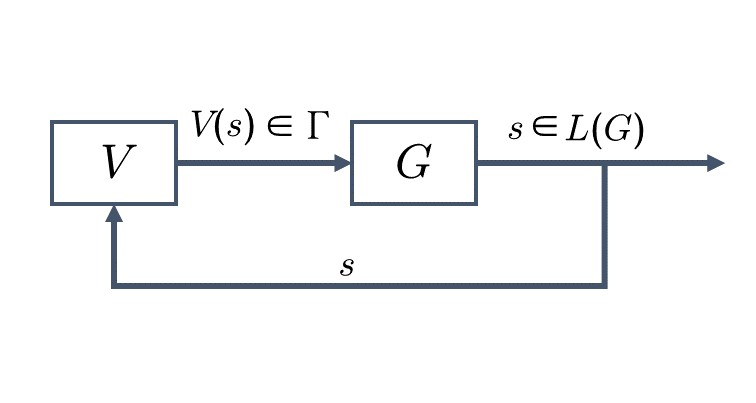
\includegraphics[scale=0.45]{figures/Feedback_Control_Loop.jpg}
    \caption{フィードバック制御ループ}
    \label{fig:Feedback_Control_Loop}
\end{figure}

\begin{enumerate}
    \item $G$は事象列$s \in L(G)$を生成する.
    \item $s$に対して,スーパーバイザ$V$が制御パターン$V(s) \in \Gamma$を生成する.
    \item 次の2つを満たした場合, $G$は$s$に続く$\sigma$を生成する.
    \begin{enumerate}
        \renewcommand{\theenumii}{\roman{enumii}}
        \item $\sigma \in V(s)$($V$に許可された$\sigma$)
        \item $s\sigma \in L(G)$($G$で,$s$の後物理的に起こり得る$\sigma$)
        \end{enumerate}
  \item $s\sigma$を$s$に代入し,$1$へ戻り繰り返す.
\end{enumerate}

$V/G$によって生み出される言語は$L(V/G)$とかき,以下のように定義する.
\begin{enumerate}
    \renewcommand{\labelenumi}{(\roman{enumi})}
    \item $\epsilon \in L(V/G)$
    \item $s \in L(V/G)\ \&\ \sigma \in V(s)\ \&\ s\sigma \in L(G) \Rightarrow s\sigma  \in L(V/G)$
    \item (i),(ii)以外の事象列は$L(V/G)$に属しない.
\end{enumerate}

また$L(V/G)$について三式が成り立つ.

\begin{eqnarray}
    L(V/G)&\neq&\emptyset\\L(V/G)&=&\overline{L(V/G)}\\L(V/G)&\subseteq&L(G)
\end{eqnarray}


\subsection{可制御性}

制御要求を満たす言語$K \subseteq L_m(G)$をおく.$V/G$のマーク言語$L_m(V/G)$を以下のように定義する.
$$L_m(V/G) \coloneqq L(V/G) \cap K$$
また,このときの$V$を$(K, G)$に対するマーキングスーパーバイザ制御と呼ぶ.
$\overline{L_m(V/G)} = L(V/G)$のとき,$V$はノンブロッキングである.そして,$K$が制御可能のときかつその時に限り,ノンブロッキングである$(K,G)$に対する$V$が存在する.制御可能であるというのは,$\overline{K}$に含まれるすべての事象列について
\begin{equation}
    \overline{K}\Sigma_u\cap L(G)\subseteq\overline{K}
\end{equation} 
が成り立つときの$K$をいう.
%言い換えれば制御可能とは,不可制御事象が生起したとしても受理状態まで到達可能であることをいう.%ここがまだ直せてない


制御可能であれば,制御要求を満たすスーパーバイザが存在する.つまりノンブロッキングなマーキングスーパーバイザを作ることができるかどうかは可制御性に依存している.


\subsection{最大許容スーパーバイザ}

$K$の制御可能な部分言語すべての集合を$C(K)$とかく.
\begin{equation}
    C(K)\coloneqq\{K^\prime\subseteq K\mid\overline{K^\prime}\Sigma_u\cap L(G)\subseteq\overline{K^\prime}\}
\end{equation}

また,以下のような式で表せる,$C(K)$の要素のうちすべての$K^\prime$を含んでいる最大要素$supC(K)$を定義する.

\begin{equation}
    supC(K) \coloneqq \bigcup\{K^\prime\mid K^\prime\in C(K)\}
\end{equation}

制御要求の言語$E(E\subseteq\Sigma^\ast)$が与えられて$K=E\cap L_m(G)\subseteq L_m(G)$とし,$K_{sup}=supC(K)$($\neq\emptyset$)であったとする.このとき,
\begin{equation}
    L_m(V_{sup}/G)=K_{sup}
\end{equation}
となる$(K_{sup},G)$に対するノンブロッキングなマーキングスーパーバイザ制御$V_{sup}$が常に存在する.またこのときのスーパーバイザを最大許容スーパーバイザとよぶ.
